% technical background

% sample latex/latex2e file with lots of math, tables, figures, etc
% useful for writing papers
% genuine finger-typed files by Christina C. Christara

\documentclass[12pt]{article}
% \documentclass[12pt]{mypaper}

%\linespread{1.1} % for more than single spacing

% take more advantage of the size of paper
\addtolength{\topmargin}{-2cm}
\addtolength{\textheight}{4cm}
\addtolength{\evensidemargin}{-2cm}
\addtolength{\oddsidemargin}{-2cm}
\addtolength{\textwidth}{4cm}

% some standard packages
\usepackage{times}
\usepackage{graphics}
\usepackage{graphicx}
\usepackage{caption}
\usepackage{subcaption}
% \usepackage{subfigure, epsfig}
\usepackage{rotate}
\usepackage{amssymb}
\usepackage{amsmath}
\usepackage{natbib} % bib
\usepackage{tikz} % neural networks
\usetikzlibrary{matrix,chains,positioning,decorations.pathreplacing,arrows}


\setlength{\parskip}{3mm}
% convenient abbreviations
\newcommand{\de}{\partial}
\newcommand{\mb}{\mathbf}

\begin{document}


\Large
{\bf Background}

\normalsize
This document will explore the technical details of a feed-forward 
neural network, and an application for recognizing hand-written digits.

% neural networks background


In the simplest case, neural networks can be reduced to 
a generalized linear model (GLM),
where the prediction is a linear combination of inputs
but passed through a non-linear function:
%
\begin{equation}
	f(\mb{x},\mb{w}) = g\left( \sum_{i=1}^N w_i x_i \right)
\end{equation}
%
\indent Here $g(\cdot)$ is a non-linear function, 
with $\mb{x}$ is an $N$ dimensional input vector,
and $\mb{w}$ is the weight vector.
Common choices of $g(\cdot)$, also known as activation functions,
for neural networks 
include the logistic (sigmoid) function, the hyperbolic tangent function, 
and the rectified linear unit (ReLU):
%
\begin{equation}
\begin{aligned}
	g_{\text{logistic}}(z) &= \frac{1}{1+e^{-z}} \\
	g_{\text{tanh}}(z) &= \tanh(z) = \frac{1 - e^{-2z}}{1 + e^{-2z}}\\
	g_\text{ReLU}(z) &= \max(z,0)
\end{aligned}
\end{equation}
%
% \indent 
where in the case of GLMs $z$ denotes the linear combination
$\sum_{i=1}^N w_i x_i$.
Notice all of these functions have simple derivatives,
and specifically logistic and hyperbolic tangent functions 
are monotonic and bounded by their horizontal asymptotes at infinities,
which makes them great choices for binary classification problems.

Graphically, this can be represented by a series of 
input nodes $\{x_i\}$ connected to an output node $f$,
with weights $\{w_i\}$ on the connections.

\def\layersep{2.5cm}
\begin{figure}[h]
\centering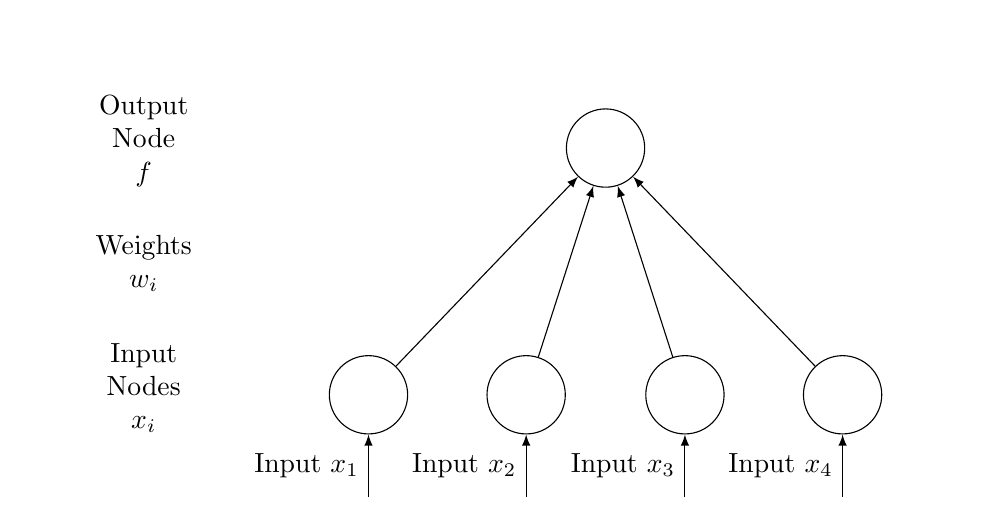
\begin{tikzpicture}[
plain/.style={
  draw=none,
  fill=none,
  },
net/.style={
  matrix of nodes,
  nodes={
    draw,
    circle,
    inner sep=10pt
    },
  nodes in empty cells,
  column sep=0pt,
  row sep=-1cm
  },
>=latex
]

\matrix[net] (mat)
{
|[plain]| \parbox{1.2cm}{\centering Output Node\\$f$} & |[plain]| & 
    |[plain]| & |[plain]| & |[plain]| & & |[plain]| & |[plain]| & |[plain]| 
    & |[plain]| \\
|[plain]| \parbox{1.3cm}{\centering Weights\\$w_{i}$}
    &|[plain]| &|[plain]| &|[plain]| &|[plain]| &
    |[plain]| &|[plain]| &|[plain]| &|[plain]| &|[plain]| \\
|[plain]| \parbox{1.3cm}{\centering Input Nodes\\$x_i$} & 
    |[plain]| & & |[plain]| & & |[plain]| & & |[plain]| &\\
};
\foreach \ai [count=\mi ]in {3,5,7,9}
  \draw[<-] (mat-3-\ai) -- node[left] {Input $x_\text{\mi}$} +(0cm,-1.3);
\foreach \ai in {6}
{\foreach \aii in {3,5,7,9}
  \draw[<-] (mat-1-\ai) -- (mat-3-\aii);
}
\end{tikzpicture}

\caption{\label{fig:GLM}
A generalized linear model represented in graphical form.
In a neural network, this is also referred to as a single neuron.
}
\end{figure}

%formatting
\pagebreak

A general feed-forward neural network is defined by recursive GLMs
with different weights.
For example, a neural network with two hidden layers
(three layers of recursion) is defined as:
%
\begin{equation}
\begin{aligned}
	h^{(1)}_j &= g^{(1)}
		\left(\sum_{i=1}^{N^{(1)}} w_{ij}^{(1)} x_i \right) \\
	h^{(2)}_k &= g^{(2)}
		\left(\sum_{j=1}^{N^{(2)}} w_{jk}^{(2)} h_j^{(1)} \right) \\
	f_l &= g^{(3)}
		\left(\sum_{k=1}^{N^{(3)}} w_{kl}^{(3)} h_k^{(2)} \right)
\end{aligned}
\end{equation}
%
where $g(\cdot)^{(\alpha)}$ is some activation function,
$h^{(\alpha)}_j$ denotes the $j^\text{th}$ node of the $\alpha^\text{th}$ 
hidden layer,
$w_{ij}^{(\alpha)}$ denotes the weight for the connection of 
the $i^\text{th}$ node of the $\alpha^\text{th}$ layer to 
the $j^\text{th}$ node of the $(\alpha+1)^\text{th}$ layer,
and $N^{(\alpha)}$ denotes the number of nodes in the $\alpha^\text{th}$ layer.
Additionally, let $N^{(4)}$ be the number of 
output nodes $f_l$.
Here we also note that $N^{(1)}$ is the number of input nodes.

Graphically, this structure has a very clear representation:
%
\def\layersep{2.5cm}
\begin{figure}[h]
\centering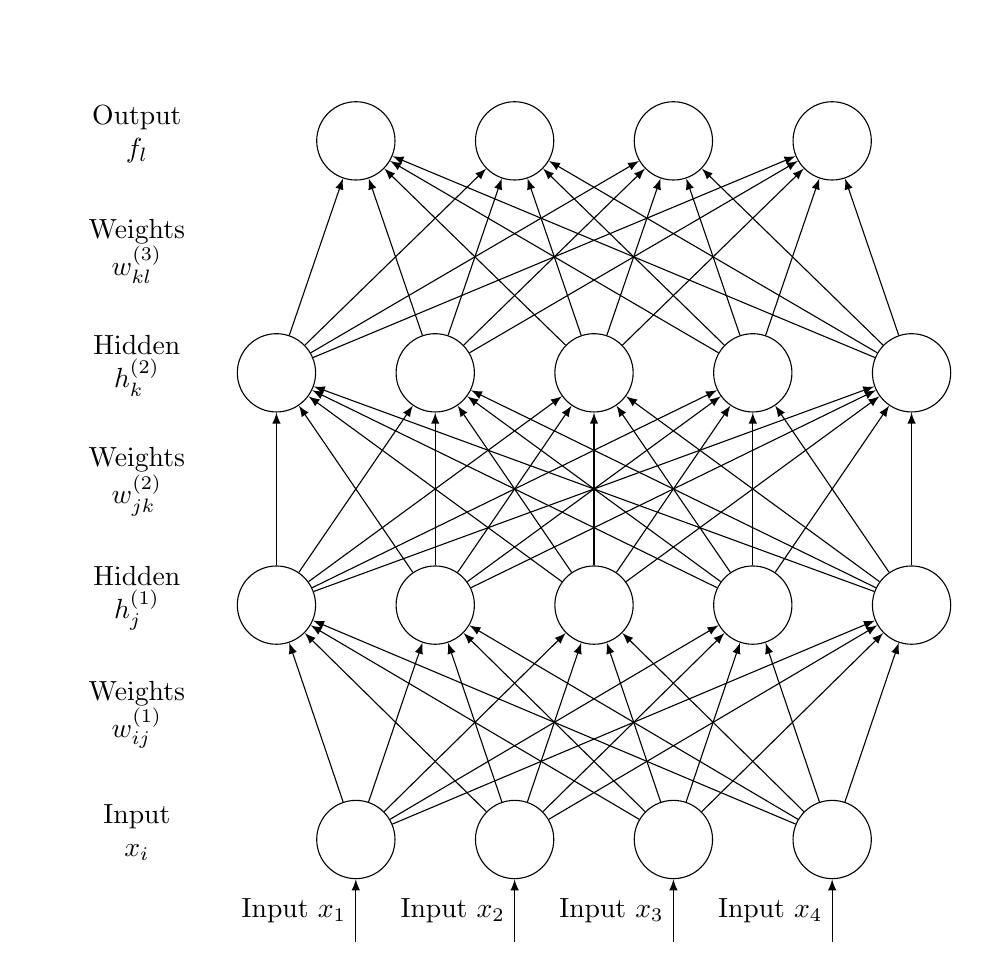
\begin{tikzpicture}[
plain/.style={
  draw=none,
  fill=none,
  },
net/.style={
  matrix of nodes,
  nodes={
    draw,
    circle,
    inner sep=10pt
    },
  nodes in empty cells,
  column sep=0pt,
  row sep=-1cm
  },
>=latex
]

\matrix[net] (mat)
{
|[plain]| \parbox{1.3cm}{\centering Output\\$f_l$} & 
    |[plain]| & & |[plain]| & & |[plain]| & & |[plain]| &\\
|[plain]| \parbox{1.3cm}{\centering Weights \\$w_{kl}^{(3)}$}\\
    % &|[plain]| &|[plain]| &|[plain]| &|[plain]| &
    % |[plain]| &|[plain]| &|[plain]| &|[plain]| &|[plain]| \\
|[plain]| \parbox{1.2cm}{\centering Hidden\\$h_k^{(2)}$} & & 
    |[plain]| & & |[plain]| & & |[plain]| & & |[plain]| & \\
|[plain]| \parbox{1.3cm}{\centering Weights \\$w_{jk}^{(2)}$}
    &|[plain]| &|[plain]| &|[plain]| &|[plain]| &
    |[plain]| &|[plain]| &|[plain]| &|[plain]| &|[plain]| \\
|[plain]| \parbox{1.2cm}{\centering Hidden\\$h_j^{(1)}$} & & 
    |[plain]| & & |[plain]| & & |[plain]| & & |[plain]| & \\
|[plain]| \parbox{1.3cm}{\centering Weights \\$w_{ij}^{(1)}$}
    &|[plain]| &|[plain]| &|[plain]| &|[plain]| &
    |[plain]| &|[plain]| &|[plain]| &|[plain]| &|[plain]| \\
|[plain]| \parbox{1.3cm}{\centering Input\\$x_i$} & 
    |[plain]| & & |[plain]| & & |[plain]| & & |[plain]| &\\
};
\foreach \ai [count=\mi ]in {3,5,7,9}
  \draw[<-] (mat-7-\ai) -- node[left] {Input $x_\text{\mi}$} +(0cm,-1.3);
\foreach \ai in {3,5,7,9}
{\foreach \aii in {2,4,...,10}
  \draw[<-] (mat-1-\ai) -- (mat-3-\aii);
}
\foreach \ai in {2,4,...,10}
{\foreach \aii in {2,4,...,10}
  \draw[<-] (mat-3-\ai) -- (mat-5-\aii);
}
\foreach \ai in {2,4,...,10}
{\foreach \aii in {3,5,7,9}
  \draw[<-] (mat-5-\ai) -- (mat-7-\aii);
}
\end{tikzpicture}

\caption{\label{fig:NN}
A generalized feed-forward neural network with two hidden layers.
}
\end{figure}

% formatting
\pagebreak 

While most GLMs do not admit a closed-form solution,
a satisfactory optimization can be achieved by the gradient descent method.
In the neural network case,
the optimization becomes more difficult as
the number of parameters increase with the number of nodes and layers.
However, we can still apply the gradient descent method
and find a local optimum for the simpler neural networks.

Suppose we have a dataset $\mathcal{D} = \{\mb{x}^{[n]}, 
\mb{y}^{[n]}\}, n \in \mathbb{N}$,
and we want to find a model $f(\mb{x},\mb{w})$ such that 
it is the ``closest'' to $\mb{y}$.
If the error function $E(f,\mb{y})$
and the model $f(\mb{x},\mb{w})$ are differentiable
with respect to $\mb{w}$,
the model can be optimized by gradient descent.
In other words, for any randomly initialized $\mb{w}^0$,
an improvement $\mb{w}^{k+1}$ can be obtained by making a 
small modification
in the direction of the gradient with respect to $\mb{w}^k$ :
%
\begin{equation}
	\mb{w}^{k+1} = \mb{w}^{k} - \eta \; \nabla_{\mb{w}^k} 
					E\left(f(\mb{x},\mb{w}^k),\mb{y}\right)
\end{equation}
%
where $\eta > 0$ is hyper-parameter controlling the change of 
each optimization iteration, commonly called the learning rate.
Note $\eta$ is not part of the final model $f(\mb{x},\mb{w})$,
but it will significantly influence optimization.

In the two hidden layer neural network previously,
a derivative with respect to any weight 
$w_{ij}^{(\alpha)}$ can be found
by applying the chain rule to the derivatives.
For example the derivative with respect to $w_{jk}^{(2)}$ :
%
\begin{equation}
\begin{aligned}
	\text{let } z_j^{(\alpha)} &= 
		\sum_{i=1}^{N^{(\alpha)}} w_{ij}^{(\alpha)} h_i^{(\alpha-1)} \\
	\text{then } \frac{\de E}{\de w_{jk}^{(2)}} &= 
		\sum_{l=1}^{N^{(4)}} \frac{\de E}{\de f_l}
		\frac{\de f_l}{\de z_l^{(3)}}
		\frac{\de z_l^{(3)}}{\de h_k^{(2)}}
		\frac{\de h_k^{(2)}}{\de z_k^{(2)}}
		\frac{\de z_k^{(2)}}{\de w_{jk}^{(2)}} \\
	&=
		\sum_{l=1}^{N^{(4)}} \frac{\de E}{\de f_l}
		\frac{\de g^{(3)}(z_l^{(3)}) } {\de z_l^{(3)}}
		w_{kl}^{(3)}
		\frac{\de g^{(2)}(z_k^{(2)}) } {\de z_k^{(2)}}
		h_j^{(1)} .
\end{aligned}
\end{equation}
%
% \indent 
Recall $g^{(\alpha)}(\cdot)$ is selected to have a simple derivative,
making the complex appearing gradient term above easy to compute.

A common technique to improve speed of convergence 
is by adding momentum.
Instead of letting the gradient dictate the change in $\mb{w}^k$,
the idea is to let the gradient dictate the rate of change.
If $\mb{w}^k$ is interpreted as a coordinate,
and each optimization iteration as velocity,
momentum can be seen as using the gradient as acceleration. 
This allows the optimization to accumulate speed in 
a consistent direction of the gradient, 
while making it harder to slow down and 
converge to a poor local minimum.
The formulation starts with a velocity vector $\mb{v}^0$
initialized to zero, and the rest in similar:
%
\begin{equation}
\begin{aligned}
	\mb{v}^{k+1} &= \theta \mb{v}^{k} - \eta \; \nabla_{\mb{w}^k} 
				E\left(f(\mb{x},\mb{w}^k),\mb{y}\right) \\
	\mb{w}^{k+1} &= \mb{w}^{k} + \mb{v}^{k+1}
\end{aligned}
\end{equation}
%
where $\theta \in [0,1]$ is the hyper-parameter 
deciding the preservation of momentum.
Here choosing a larger $\theta$ would result in a stronger 
preservation of the velocity vector $\mb{v}$,
which then improves momentum.

% formatting
\pagebreak
\noindent
\large
{\bf MNIST Hand-Written Digits}
\normalsize

The Mixed National Institute of Standards and Technology
(MNIST) dataset is a collection of images of hand-written digits
from various sources,
with each image labeled the correct digit.
The dataset contains 60,000 images for training (fitting),
and 10,000 images for testing.
The images are 28x28 in resolution,
hence making $N^{(1)} = 784$ dimensions in input.

The data labels are changed to use the 1-of-K encoding scheme,
where the label $\mb{y}$ is a binary vector of size K,
with only one element taking a value of one.
In this case, given 10 possible digits,
we have a vector of size $N^{(4)} = 10$.
For example, a possible scheme can label the digit ``$3$'' 
using the vector $[0,0,1,0,\ldots]$ where 
only the $3^\text{rd}$ index is a ``$1$''.

To best model this type of label vector,
the softmax function is chosen for the output layer:
%
\begin{equation}
	f_l = 
	g^{(3)}(z_l^{(3)}) = \frac{\exp(z_l^{(3)})}
		{\sum_{k=1}^{N^{(4)}} \exp(z_k^{(3)})}
\end{equation}
%
\indent As a result the sum of $f_l$ adds up to one,
and the most optimal output is exactly the 1-of-K encoded label.
If $f_l$ is modeled as the probability of the image being digit $l$,
suppose the correct digit is $m$,
then the likelihood of making the correct prediction is:
%
\begin{equation}
  L(\mb{f},\mb{y}) = f_m = \prod_{l=1}^{N^{(4)}} f_l \, ^{y_l}
\end{equation}
%
since $y_m = 1$ is the only non-zero term in the label vector.
We can then define the error function as negative log-likelihood:
%
\begin{equation}
% \begin{aligned}
	E(\mb{f},\mb{y}) 
		= - \log \prod_{l=1}^{N^{(4)}} f_l \, ^{y_l}
		= - \sum_{l=1}^{N^{(4)}} y_l \log f_l
% \end{aligned}
\end{equation}
%
where $N^{(4)}$ is the number of output nodes, 
and minimizing $E$ is equivalent to maximizing likelihood.
Note taking the logarithm creates an error function with much
simpler derivative, 
hence simplifying the gradient descent method.

In the following experiment, 
a two hidden layer neural network is used to model the MNIST digits.
We used $N^{(2)} = N^{(3)} = 1000$ nodes in the hidden layers, 
creating a structure of 784-1000-1000-10 
$\left( N^{(1)} - N^{(2)} - N^{(3)} - N^{(4)} \right)$
nodes in each layer.
We also chose 
$g^{(1)}(\cdot) = g^{(2)}(\cdot) = g_\text{ReLU}(\cdot)$ 
in the hidden layers,
and softmax for the output layer.
The hyper parameters were chosen as $\eta = 10^{-5}$
and $\theta = 0.9$.
We also chose to update the weight vector $\mb{w}^k$ once
for every 100 samples of digits,
also known as a mini-batch.

After training (optimizing) for 50 epochs,
with each epoch denoting one complete run through of the training 
dataset,
we reach a test error rate of $16\%$ (Figure \ref{fig:mnist_err}).
%
\begin{figure}[h]
\centering
\begin{subfigure}{.45\textwidth}
  \centering
  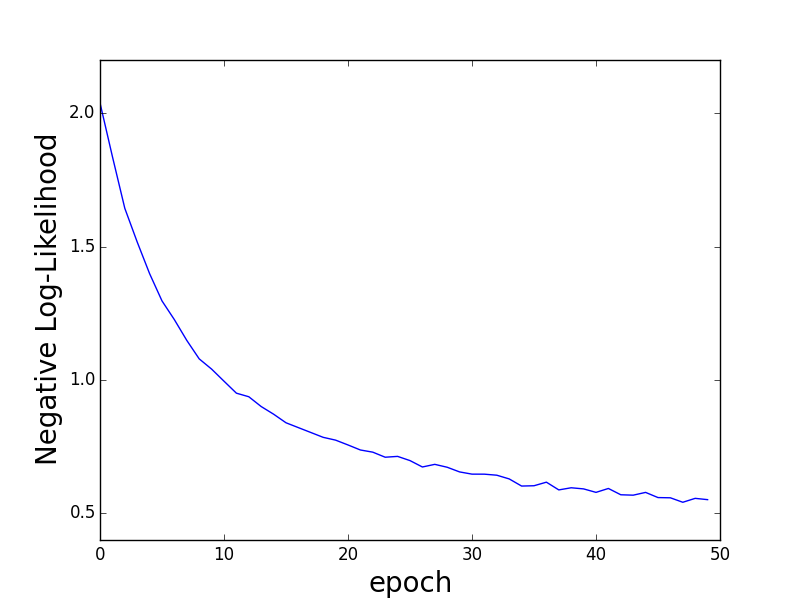
\includegraphics[width=\linewidth]{fig_mnist_nll.png}
  \caption{The negative log-likelihood}
  \label{fig:mnist_nll}
\end{subfigure}%
\begin{subfigure}{.45\textwidth}
  \centering
  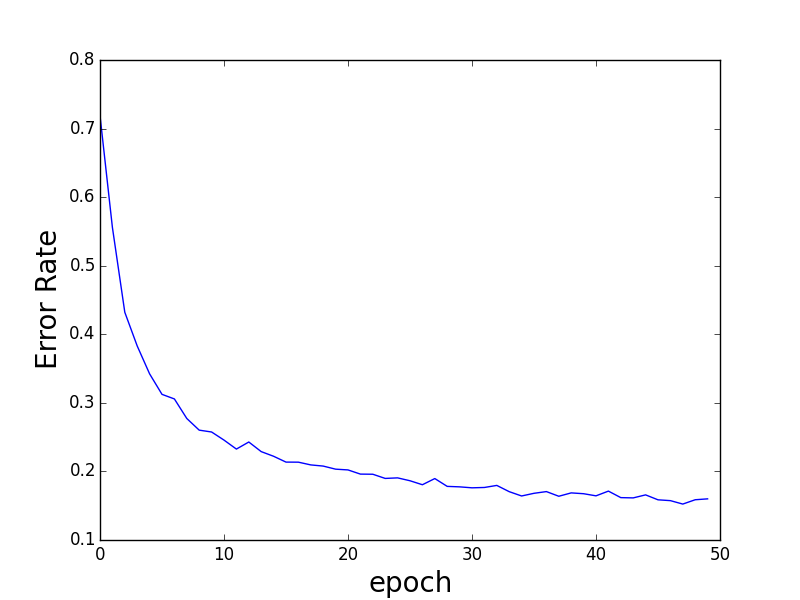
\includegraphics[width=\linewidth]{fig_mnist_err.png}
  \caption{The classification error rate}
  \label{fig:mnist_err}
\end{subfigure}
\caption{MNIST hand-written digits modeled using a two hidden
  layer neural network, with negative log-likelihood and
  classification error rate computed after each epoch.}
\label{fig:mnist_results}
\end{figure}
%
By increasing the number of epochs and a few minor modifications,
this model could potentially reach error rates as low as $2\%$.
However, this will not be explored since it is not
the main purpose of this document,
and optimization can be very time consuming due to computation.

% It is important to note that the activation function chosen is ReLU, 
% which is not easy to incorporate due within a 
% restricted Boltzmann machine context due to an unbounded range.
% However, a recently introduced method called 
% general adversarial networks can be used instead using the ReLU functions
% in alternative to restricted Boltzmann machines.
% This will be explored further in future discussions.

While the technique is more than a sufficient solution 
for recognizing hand-written digits,
naively applying gradient descent to more complex 
neural networks tend to have poor results.
Alternative methods will be discussed in the next section 
in order to address this problem.

Also note this type of neural networks is feed-forward, 
which mean it is limited to only supervised type problems
where the data structure is consistent 
and a prediction target (label) is provided for each sample.
For a collaborative filtering type problem,
the inference is often made within the data structure itself, 
which makes an unsupervised learning problem.
Feed-forward neural networks also fail to fully utilize 
the datasets that are partly labeled, 
known as semi-supervised problems.
These problems would require other variations of neural networks
with different methods for inference.







% background on restricted Boltzmann machines

\noindent
\large
{\bf Restricted Boltzmann Machines}
\normalsize

Motivated by optimization of a more complex neural network
and prediction of an unsupervised or semi-supervised learning problem
such as collaborative filtering,
it turns out that restricted Boltzmann machines can address 
all of these problems. 
A RBM is a Markov random field in a bipartite graph structure,
where there are two layers of nodes,
no internal connections within each layer.
One layer of nodes contain the input $\mb{x}$,
while the other contain hidden values $\mb{h}$.
%
\def\layersep{2.5cm}
\begin{figure}[h]
\centering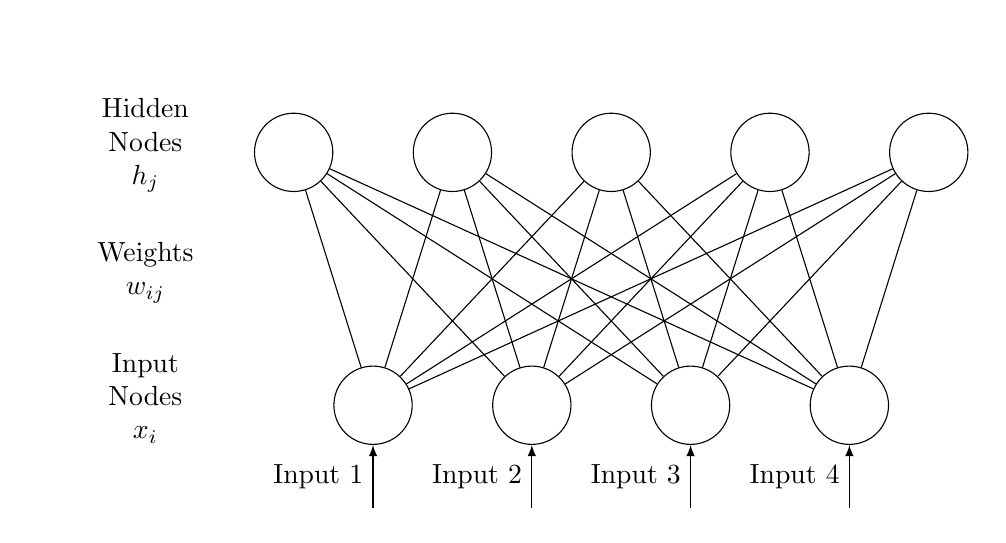
\begin{tikzpicture}[
plain/.style={
  draw=none,
  fill=none,
  },
net/.style={
  matrix of nodes,
  nodes={
    draw,
    circle,
    inner sep=10pt
    },
  nodes in empty cells,
  column sep=0pt,
  row sep=-1cm
  },
>=latex
]

\matrix[net] (mat)
{
|[plain]| \parbox{1.3cm}{\centering Hidden Nodes $h_j$} & & 
    |[plain]| & & |[plain]| & & |[plain]| & & |[plain]| & \\
|[plain]| \parbox{1.3cm}{\centering Weights $w_{ij}$}
    &|[plain]| &|[plain]| &|[plain]| &|[plain]| &
    |[plain]| &|[plain]| &|[plain]| &|[plain]| &|[plain]| \\
|[plain]| \parbox{1.3cm}{\centering Input Nodes $x_i$} & 
    |[plain]| & & |[plain]| & & |[plain]| & & |[plain]| &\\
};
\foreach \ai [count=\mi ]in {3,5,7,9}
  \draw[<-] (mat-3-\ai) -- node[left] {Input \mi} +(0cm,-1.3);
\foreach \ai in {2,4,...,10}
{\foreach \aii in {3,5,7,9}
  \draw[-] (mat-1-\ai) -- (mat-3-\aii);
}
\end{tikzpicture}

\caption{\label{fig:RBM}
A restricted Boltzmann machine (RBM) with 4 input and 5 hidden nodes.
}
\end{figure}

Suppose the graph have $N^{(1)}$ input nodes 
and $N^{(2)}$ hidden nodes,
with weights $w_{ij}$ defined in the same way as the neural network
the bias parameters $w_{0j}$ and additionally $w_{i0}$.
Here we consider the case where $h_j$ can only take binary values,
and $\sigma_i$ as the standard deviation for each input dimension.
Finally, we can define an energy function and 
joint Boltzmann distribution for the graph:
%
\begin{equation}
\begin{aligned}
    E(\mb{x},\mb{h}|\theta) &= 
        \sum_{i=1}^N \frac{(w_{i0} - x_i)^2}{2 \sigma_i}
        - \sum_{i=1}^N \sum_{j=1}^M
             w_{ij} h_j \frac{x_i}{\sigma_i}
        - \sum_{i=j}^M w_{0j} h_j \\
    P(\mb{x},\mb{h}|\theta) &= 
        \frac{\exp\left[-E(\mb{x},\mb{h}|\theta)\right]}
        {\mathcal{Z}}
\end{aligned}
\end{equation}
%
where $\mathcal{Z}$ is the partition function normalizing 
the distribution.
































\end{document}




